\documentclass{school-22.101-notes}
\date{December 13, 2011}

\begin{document}
\maketitle

\clearpage
\topic{Gamma Interaction}
GI was not covered Fall 2011. Prof. Yip covered it over two lectures Fall 2012. Basic concepts: 
\begin{enumerate}
\item Gamma rays are electromagnetic radiations produced by nuclear transitions. These are typically \hi{photons with energies in 0.1$\sim$10 MeV}. 

\item The attenuation (either scattering or absorption, any process that removes gamma from the beam) of the intensity of a beam of gamma rays follows a true \hi{exponential} variation with respect to distance $I(x) = I_0 e^{-\mu x}$, unlike that of charged particle penetration. 

\item 3 types of GI: Compton scattering, photoelectric interaction, and pair production. Compton scattering is the most important one. These three process are independent so the total attenuation coefficient (xs) is the sum of the three. 
  \begin{table}[ht]
    \centering
    \begin{tabular}{cccc} \hline
      Target material& Absorption & Elastic Scattering & Inelastic Scattering \\  \hline \hline
      electrons & photoelectric & Thomson & Compton \\  \hline
      nucleus & x & x & x \\ \hline
      electric field around nucleus & pair production & x & x \\ \hline
    \end{tabular}
    \caption{Gamma Interaction Types}
  \end{table}

\end{enumerate}

\subtopic{Compton Scattering}
Compton scattering is the inelastic (photon loses energy) relativistic scattering by a free electron,  
which can be treat similar to neutron scattering, though we have to consider relativistic kinetics. For Compton

\begin{enumerate}
\item Basic relations. We define $E_{\gamma} = \hbar c k, \omega = 2 pi \gamma = ck$, where $c$ is speed of light and $\lambda \gamma = c$. We consider conservation of momentum and conservation of energy to get SY7 Eq.17.5 - 17.8: 
\eqn{ \lambda' - \lambda = \frac{c}{v'} - \frac{c}{v} = \frac{h}{m_e c} ( 1 - \cos \theta) }
\eqn{ \frac{\omega'}{\omega} = \frac{1}{1 + \alpha (1 - \cos \theta)}} 
where $\alpha = \frac{\hbar \omega}{m_e c^2} = \left( \frac{A-1}{A+1} \right)^2$ which characterizes the kinematics, and $\theta$ is scattering angle ($\theta = 0$ means forward scattering, $\theta = \pi$ means ...). 

\item Derivation of $\frac{\dsigma_c}{\dOmega}$ by Klein \& Nishine (1928) using relativistic QM: 
\eqn{ \frac{\dsigma_c}{\dOmega} = \frac{r_e^2}{4} \left( \frac{\omega'}{\omega} \right)^2 \left[ \frac{\omega}{\omega'} + \frac{\omega'}{\omega} - 2 + 4 \cos^2 \theta \right] }
where $\displaystyle r_e = \frac{e^2}{m_p c^2} = 2.83 \times 10^{-13} \cm$ which is the classical radius of the electron. 

\item We make two assumptions: unpolarized radiation (polarized is complex, so we ignore it), and small $\alpha$: 
\begin{enumerate}
\item For unpolarized radiation, we consider the averaging over angle $\phi$, to get SY7 Eq.17.18, 17.19.

\item For small $\alpha$ (low energy limit), Compton becomes Thompson, we can approximate $\omega' \sim \omega$ and arrive at Eq.17.16, 
\eqn{ \boxed{ \left( \frac{\dsigma_c}{\dOmega} \right)_{\mathrm{unpol}} = \frac{r_e^2}{2} (1 + \cos^2 \theta) } }
which implies that scattering is symmetric about $90\degree$. 
\end{enumerate}
Make sure you understand Fig~\ref{17.3} which says that Thompson is symmetric, and as $\alpha \up$ we become forward biased. 
\begin{figure}
  \centering
  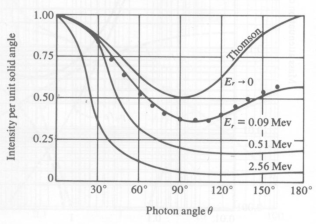
\includegraphics[width=4in]{images/ni/17.3.png}
  \caption{Angular Distribution of Compton Scattering at Various Incident Energies $E_r$. (SY7 Fig. 17.3, Heitler)} \label{17.3}
\end{figure}

\item Energy distribution of Compton electrons and photons: we combine two equations,
  \eqn{ \frac{\dsigma_c}{\dtheta} = \frac{\dsigma_c}{\dOmega} 2 \pi \sin \theta }
  \eqn{ \frac{\dsigma_c}{\domega'} = \frac{\dsigma_c}{\dtheta} \left| \frac{\dtheta}{\domega'} \right| }
  \eqn{ \frac{\dsigma_c}{\dT} = \frac{\dsigma_c}{\domega'} \left| \frac{\domega'}{\dT} \right| = \frac{\dsigma_c}{\domega'} \frac{1}{\hbar} }
where we can use $\hbar \omega' = \hbar \omega - T$. We arrive at Fig.~\ref{17.4}, where notice there is an edge effect (called Compton edge). 

\begin{figure}
  \centering
  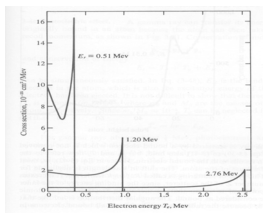
\includegraphics[width=4in]{images/ni/17.4.png}
  \caption{Energy Distribution of Compton Electrons for Several Incident Gamma-ray Energies. (SY7 Fig. 17.4, Meyerhof)} \label{17.4}
\end{figure}
\end{enumerate}

\end{document}
